\chapter{Intelligence Artificielle}

\section{Stratégies}

\subsection{Inteligence Aléatoire}

L’ IA contrôle une liste de personnages appartenant au joueur actuel,
elle va les sélectionner les uns après les autres lors de son tour 
de jeu.
Une fois un personnage sélectionné, un entier correspondant à une 
action précise est choisi au hasard parmi 6 : 1 (attaquer), 2 (se 
déplacer), 3 (utiliser un objet), 4 (défendre), 5 (utiliser une 
compétence) et 6 (passer son tour).
\\\\
Lorsqu'une action est séléctionnée on teste sa faisabilité, sinon un 
nouveau nombre est séléctionné jusqu'à ce que l'action soit valide. 
\\\\
Si l'action est possible alors elle est ajoutée à la liste des 
commandes et l'IA passe au personnage suivant.
\\\\
Si "attaquer" est choisie, une cible va être déterminée aléatoirement
parmi tout les autres personnages, y compris ceux de son équipe. Si 
la cible de l'attaque est trop éloignée alors l’attaque n’aura pas 
lieu, si la distance entre les deux personnages est suffisante alors 
l'attaque est ajoutée à la liste des commandes.
\\\\
Si "se déplacer" est choisie, le personnage sélectionné tente de se 
mouvoir sur une case aléatoire, si cela est réalisable alors le 
déplacement est ajouté à la liste des commandes.
\\\\
Si "utiliser un objet" est choisie, alors le personnage va utiliser 
un objet aléatoire de la liste des objets appartenant à son équipe, 
puis il applique l'effet sur une cible aléatoire, si l'objet est en 
quantité suffisante alors l'action est ajoutée à la liste des 
commandes.
\\\\
Si "défendre" est choisie, le personnage sélectionné se met en 
position défensive, dans le cas présent puisque l'on cherche les 
actions des personnages dans l'ordre, cette action ne peut échouer 
puisque le personnage n'a pas d'autres actions dans la liste, 
l'action "défendre" est donc ajoutée à la liste.
\\\\
Si "utiliser une compétence" est choisie, alors le personnage va 
utiliser une compétence aléatoire de la liste des compétance qu'il 
peut utiliser, puis il applique l'effet sur une cible aléatoire, si 
la distance entre lui et sa cible est inférieure à la distance 
maximum de la compétence alors la compétence est ajoutée à la liste 
des commandes.
\\\\
Si "passer son tour" est choisie, l'IA termine son tour d’action.
Lorsque passer son tour ou lorsque tout les personnages de l'équipe 
du joueur actuel ont une action, alors cela fini ainsi la liste des 
commandes, les commandes sont exécutées dans l'ordre de la liste. 
Puis c'est au tour de l'adversaire.
\\
\section{Conception Logiciel}
Le diagramme des classes UML C++ pour l'intelligence artificielle est
visible en Figure 5.1.
On divise l'intelligence artificielle en 2 classes.

\begin{itemize}

\item \textbf{AI :} C'est la classe principale, elle définie les 
méthodes qui serviront lors du polymorphisme lorsque les différentes 
IA seront appelées.

\item \textbf{RandomAI :} C'est la classe représentant l'IA 
aléatoire, elle a une fonction pour determiner la liste des actions 
des personnages controllé par l'IA (randomCommandList) et une 
fonction pour executer lancer l'IA (runAI).



\end{itemize}

\begin{figure}[H]
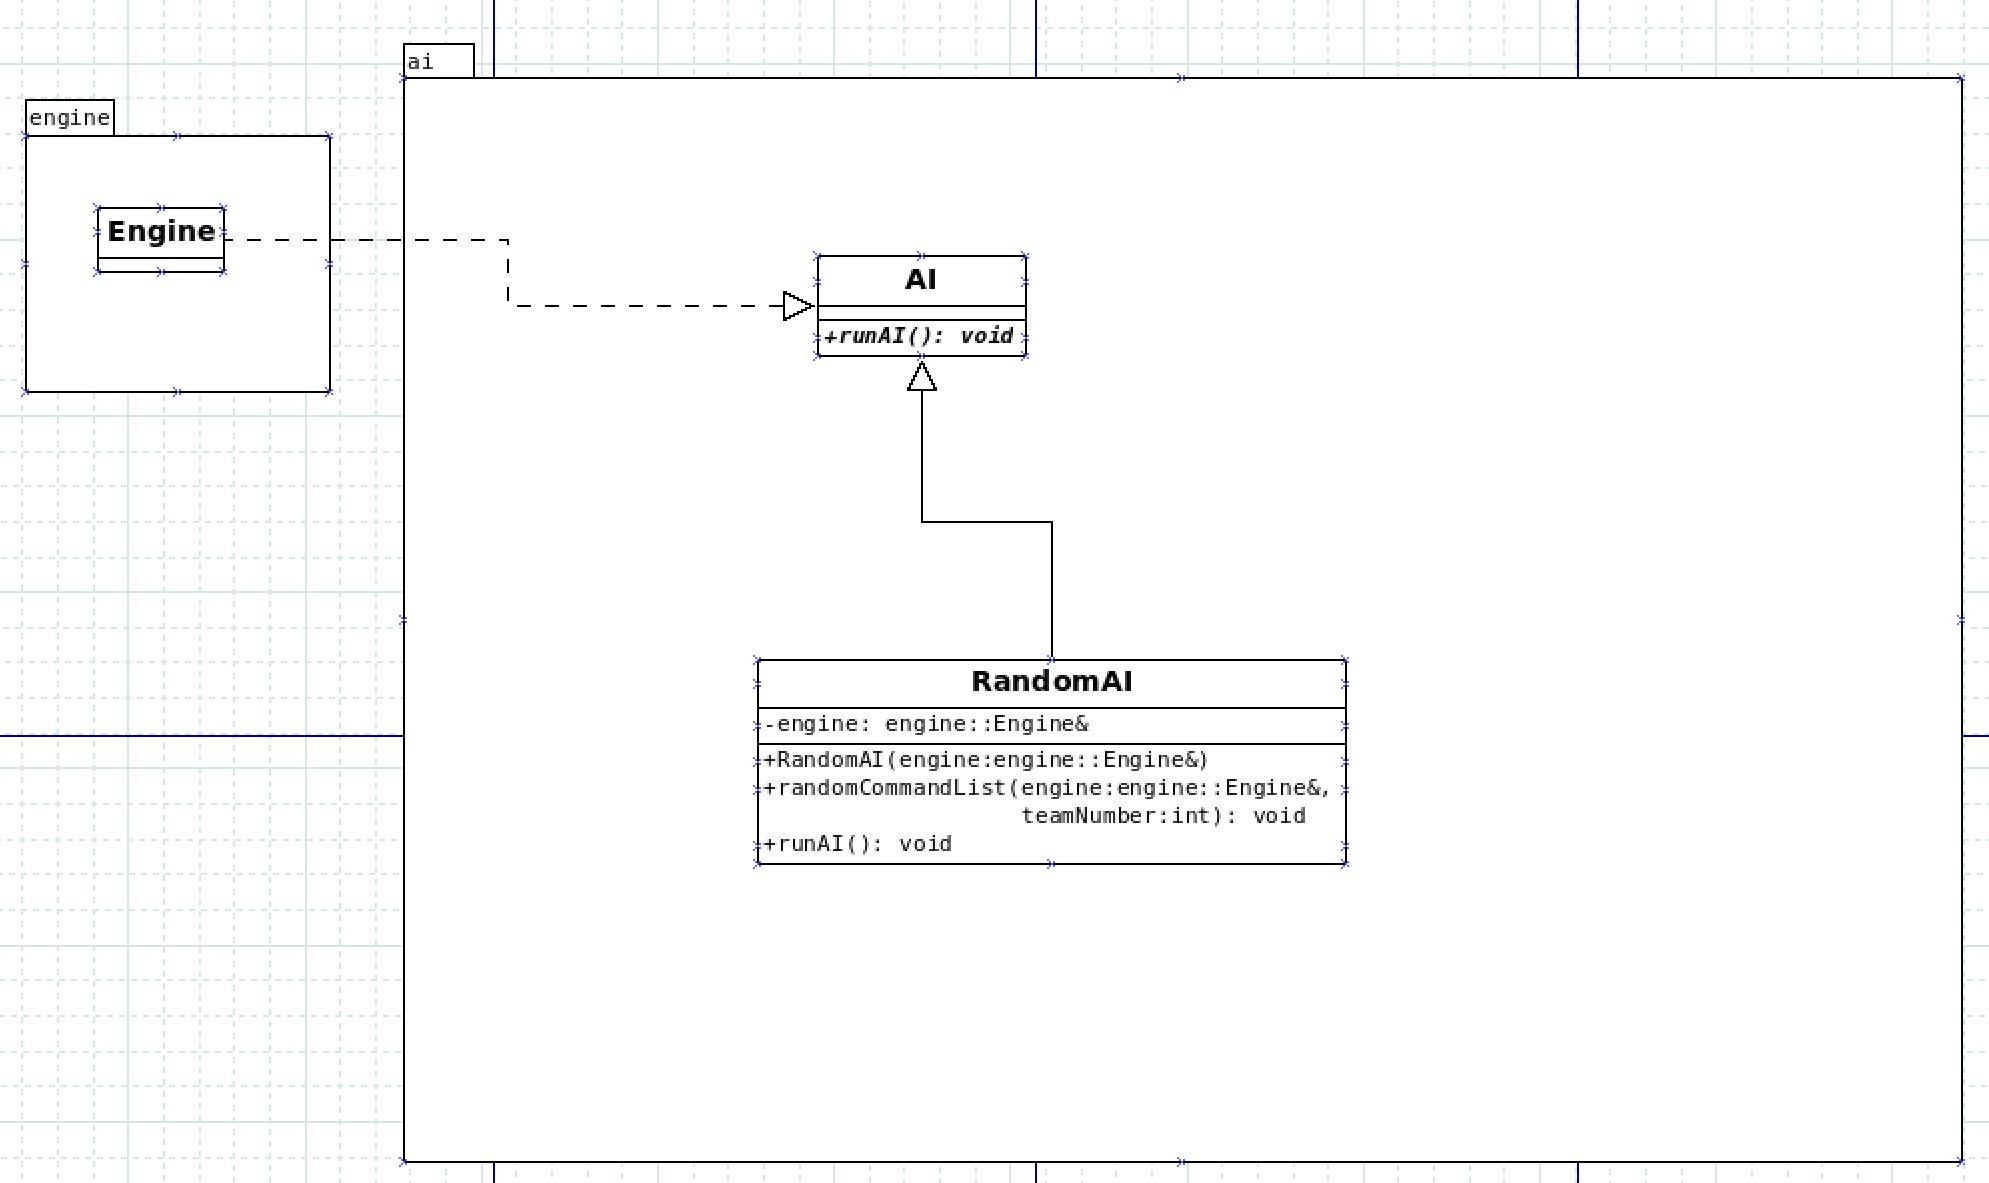
\includegraphics[width=\linewidth]{images/random_ai_dia.png}
\centering
\caption{Aperçu de ai.dia avec randomAI}
\label{fig:img3}
\end{figure}
\newpage